\section{Astrometric Calibration}
\label{sec:astrometric_calibration}


This is a quick update on astrometry quality based on data collected halfway through the \ComCam observations. It is important to note that so far only single frame astrometric calibration is being done. Doing the additional global astrometric calibration with GBDES will further improve the results presented here.


For now, metrics like AM1 (the RMS of distances between star pairs separated by 5’ across all visits on a tract) appear to be satisfactory. On average, the median value across different filters is around 10 mas, as shown in Figure \ref{AM1_plot}.

\begin{figure*}
        \centering
        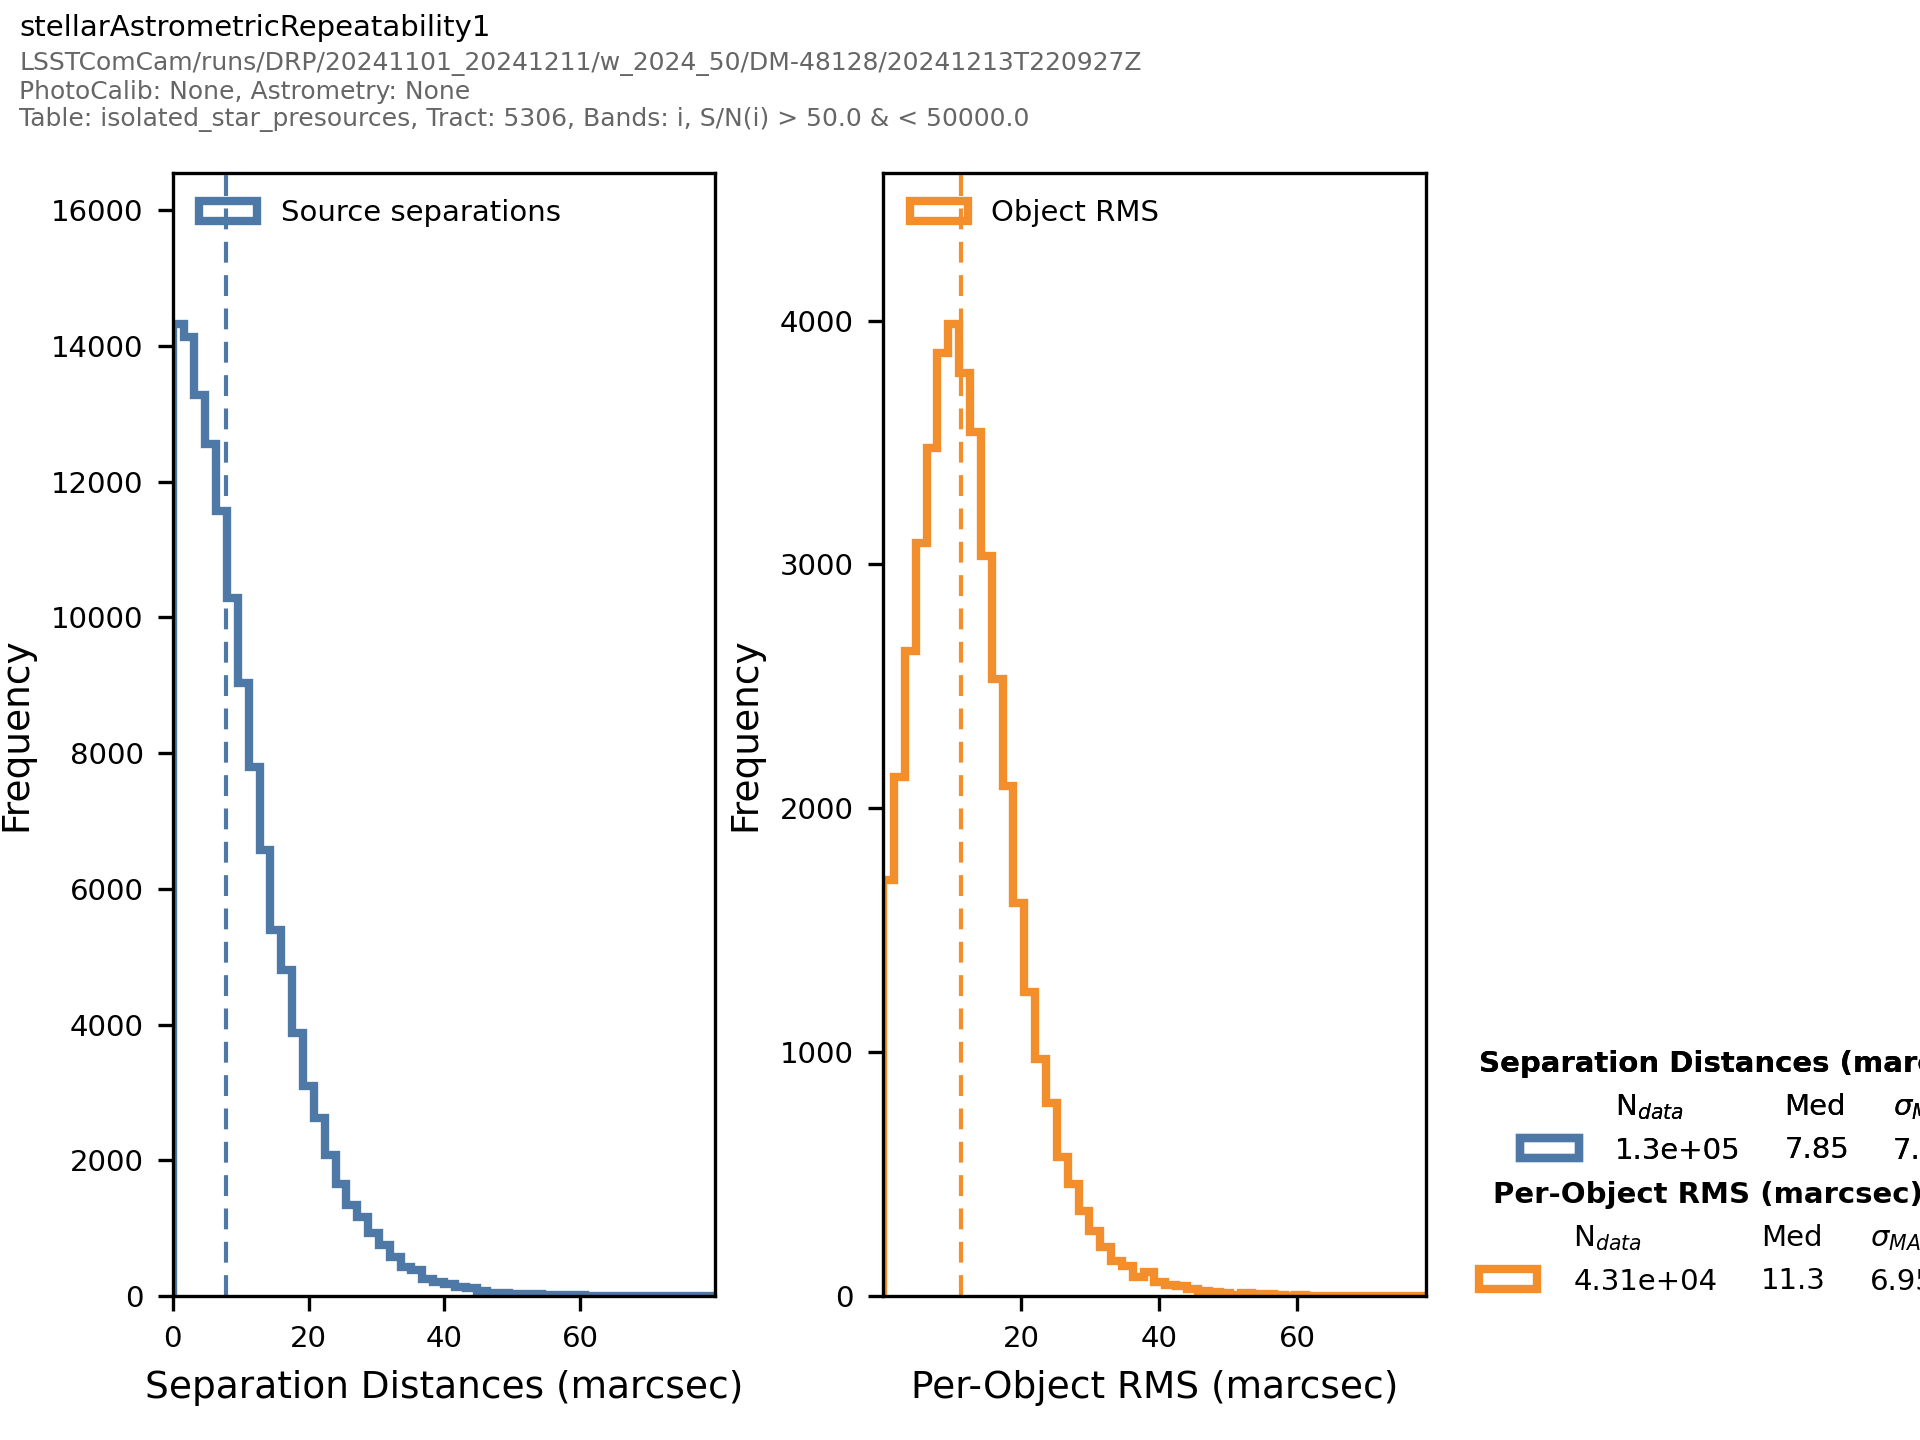
\includegraphics[scale=0.47]{figures/astrometry-f01-repeatability}
        \caption{\small Stellar Astrometric repeatability in filter I in a given tract. AM1, which is the median of the orange histogram,  is below 10 mas.}
        \label{AM1_plot}
\end{figure*}

When examining the average astrometric residuals projected across the focal plane, some structures appear to be present, as in the example below in Fig \ref{fov_astrometry_plot}. However, more data is needed to confirm whether these patterns are noise or systematic effects. It is likely that GBDES will help address these structures once it is activated. Personally, I don’t think this could be noise, but it’s fine to be noncommittal about causes here.

\begin{figure*}
        \centering
        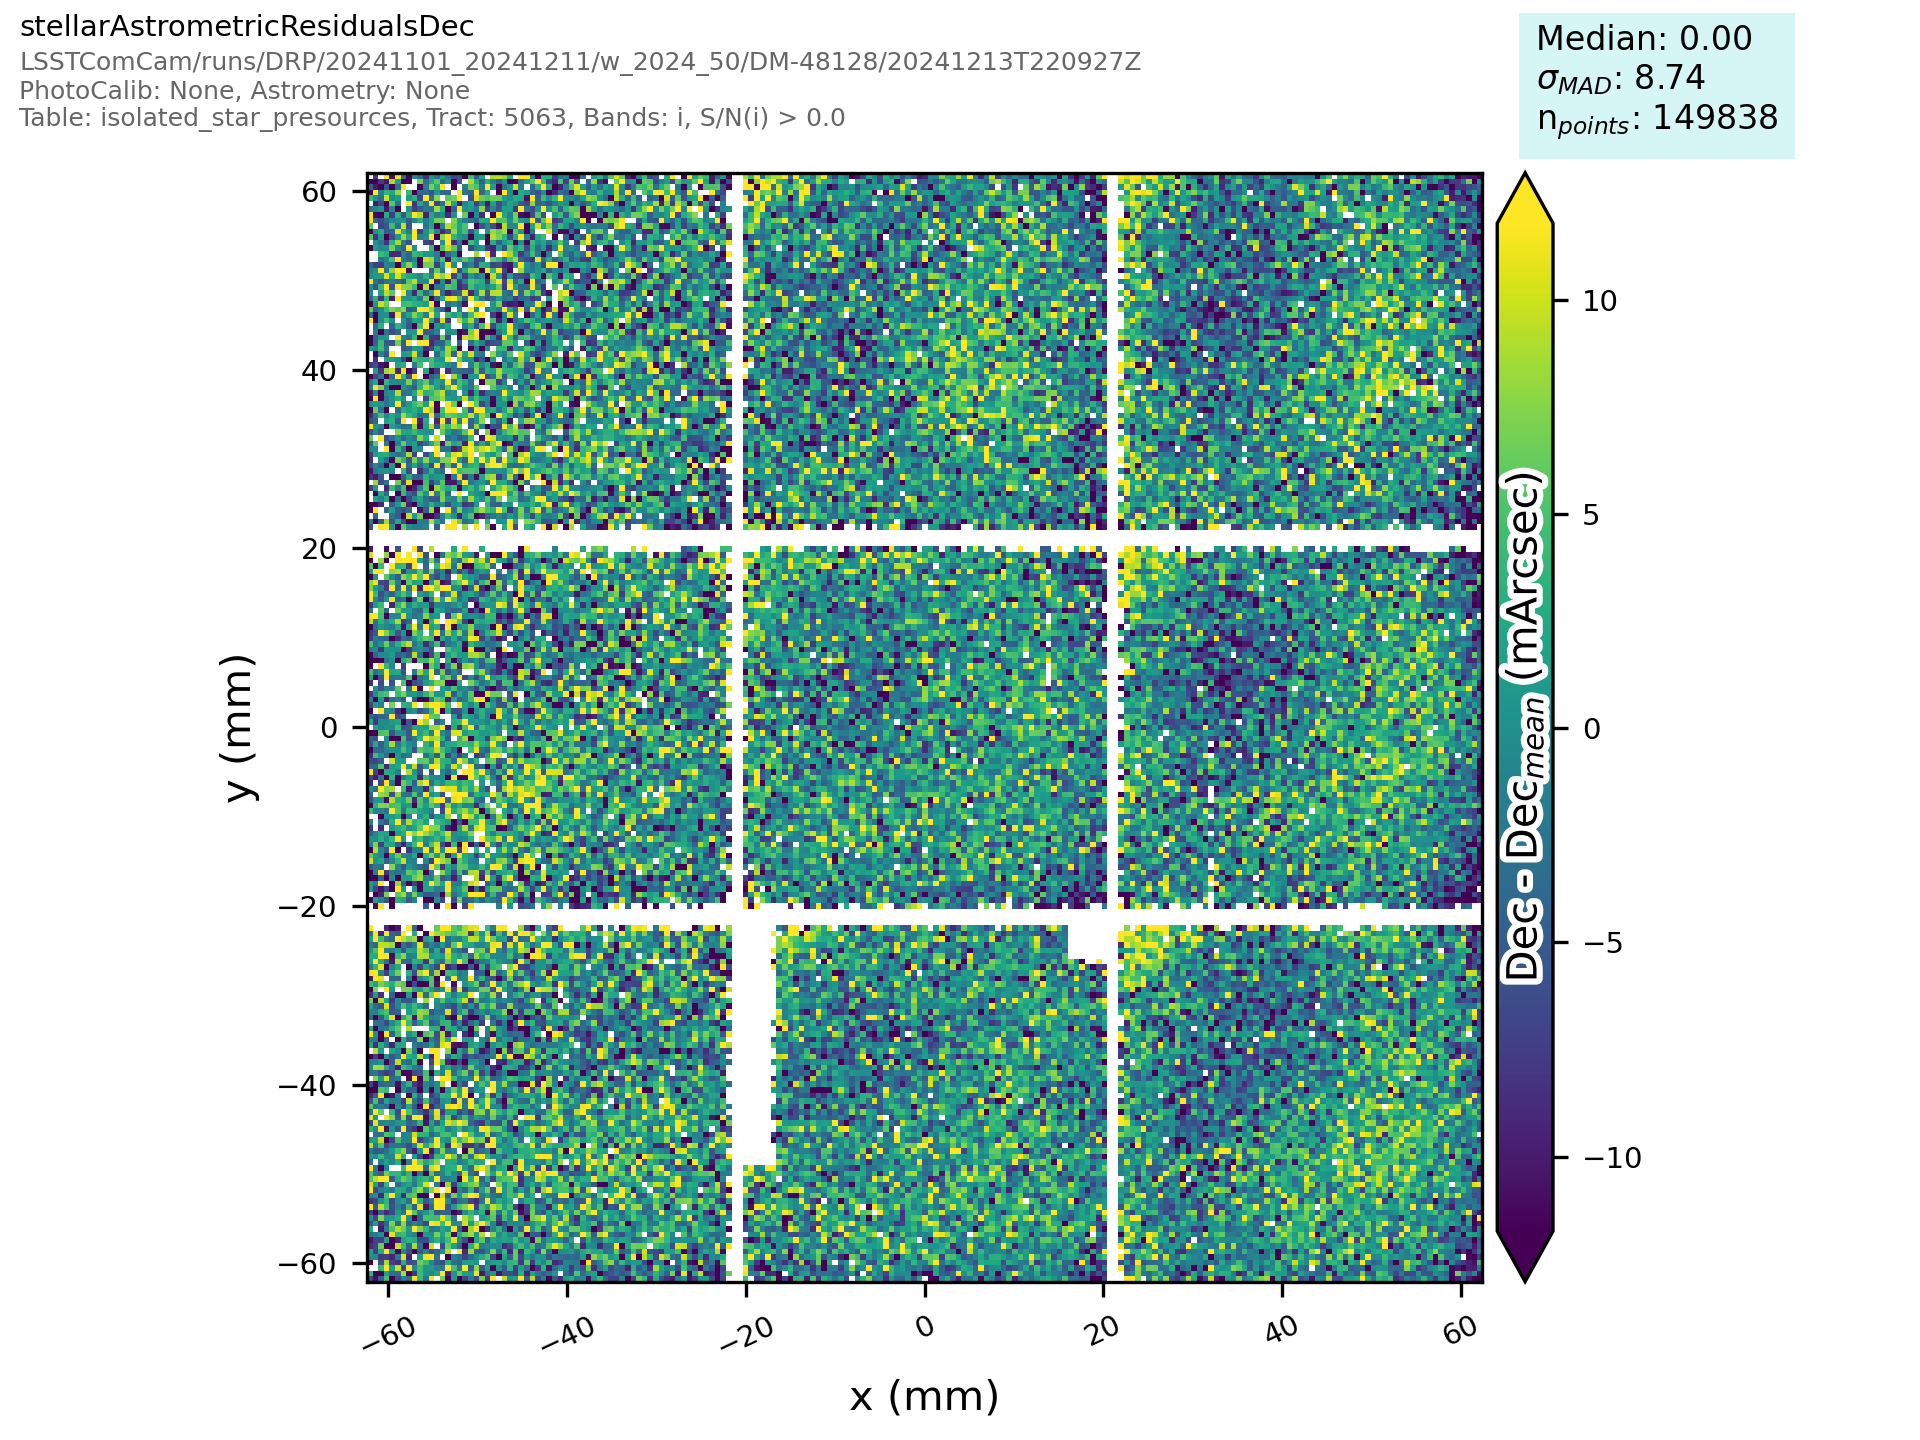
\includegraphics[scale=0.47]{figures/astrometry-f02-focal-plane-plot}
        \caption{\small Declination residuals projected in Focal plane coordinate for a given tract. Some structure looks to be present in focal plane coordinates, which will be taken into account with GBDES. }
        \label{fov_astrometry_plot}
\end{figure*}
